\documentclass{article}
    \usepackage[fontset = windowsnew]{ctex}
        \CTEXoptions[today=old]
        \ctexset{figurename=Figure}
    \usepackage{geometry}
        \geometry{left=2.54cm,right=2.54cm,top=2.54cm,bottom=2.54cm}
    \usepackage{amsmath}
    \usepackage{amsfonts}
    \usepackage{siunitx}
    \usepackage{booktabs}
    \usepackage{longtable}
    \usepackage{graphicx}
    \usepackage{subfig}
    \usepackage{float}
    \usepackage{fancyvrb}
    \renewcommand{\labelenumi}{\alph{enumi}.} % Make numbering in the enumerate environment by letter rather than number

    \title{\textbf{数字逻辑与处理器基础实验} \\ [2ex] \begin{large} \emph{32位MIPS处理器设计实验报告} \end{large} }
    \author{王晗 \\ (2013011076)}
    \date{\today}

\begin{document}
    \maketitle

    \begin{table}[htb]
        \centering
        \begin{tabular}{lr}
            Date Performed: & July 15, 2015 \\
            Partners:   & 耿天毅(2012011119) \\
                        & 陈志杰 \fbox{\begin{small}\emph{~~withdrawn~~}\end{small}} \\
        \end{tabular}
    \end{table}

    \section{实验目的}
        熟悉现代处理器的基本工作原理;掌握单周期和流水线处理器的设计方法。

    \section{设计方案}
        \subsection{总体结构}
            由于这次实验涉及的功能较多,我们将完整的CPU分成多个模块。指令存储器、寄存器堆、控制器、ALU控制器、ALU、数据存储器、UART等功能单元均在单独的Module中实现。其中指令存储器、寄存器堆、控制器、ALU控制器、ALU等单元在Single Cycle Core中实例化,作为单周期处理器的核心;数据存储器、UART和定时器、LED、七段数码管、开关在Peripheral中实现,作为处理器的外设。处理器核心和外设在顶层模块中实例化,互相通信。

            单周期CPU模块的结构关系如Figure~\ref{fig:singlecycle}所示:
            \begin{figure}[H]
                    \centering
                    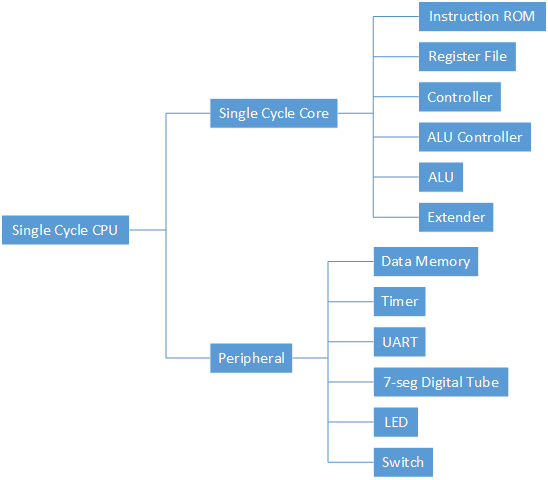
\includegraphics[width=0.62\textwidth]{images/singlecycle.png}
                    \caption{\label{fig:singlecycle}单周期处理器结构}
                \end{figure}

            对于流水线CPU,我们还在Pipeline Core中加入了流水线寄存器、冒险检测单元、数据转发单元:
            \begin{figure}[H]
                    \centering
                    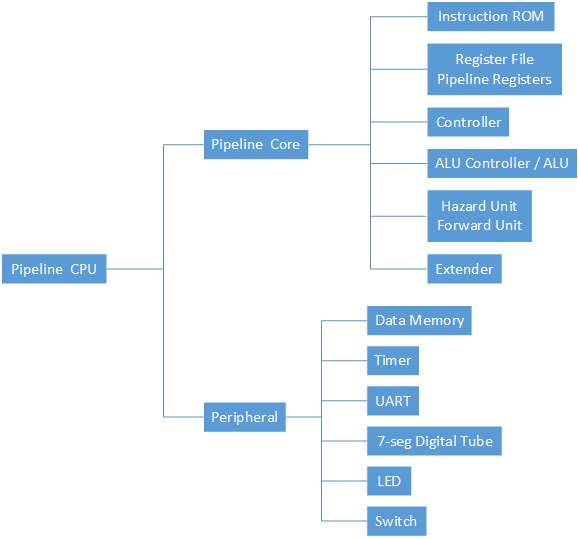
\includegraphics[width=0.62\textwidth]{images/pipeline.png}
                    \caption{\label{fig:pipeline}流水线处理器结构}
                \end{figure}

        \subsection{ALU \protect\footnote{原作者:陈志杰;修改:王晗}}
            ALU模块的结构如图所示,输入两个操作数A、B和控制信号ALUFun、Signed,在ARITH子模块中做加减法运算,CMP子模块根据ARITH模块的输出进行比较判断,LOGIC和SHIFT模块分别进行逻辑运算和移位运算,ALUFun的最高两位用于控制多路选择器的输出。
            \begin{figure}[H]
                    \centering
                    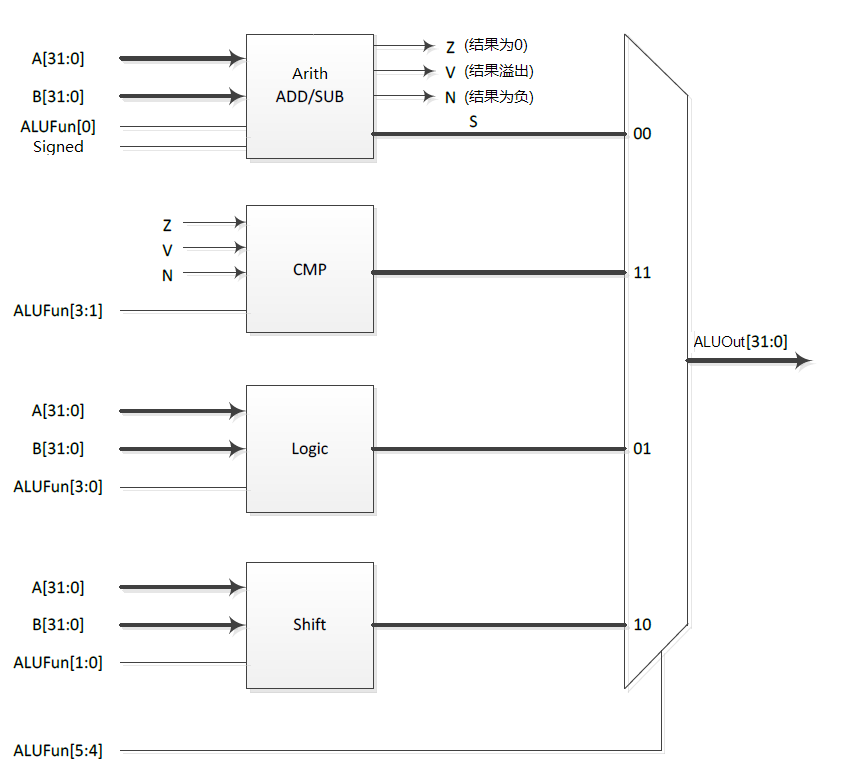
\includegraphics[width=0.62\textwidth]{images/ALU.png}
                    \caption{\label{fig:ALU}ALU结构}
                \end{figure}

            \paragraph*{ARITH模块}
            ARITH模块中包括减法和加法两个模块,加法模块直接通过+号运算,减法模块先对第二个操作数取补码,再调用加法模块做加法运算。Overflow和Negative信号的产生是ALU中的难点:
            \begin{figure}[H]
                \centering
                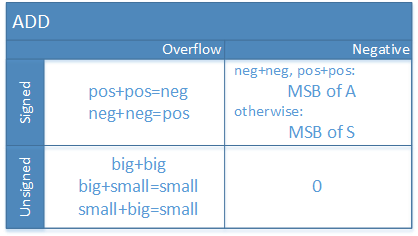
\includegraphics[width=0.5\textwidth]{images/add_v_n.png}
                \caption{\label{fig:add_v_n}ADD中的Overflow和Negative}
            \end{figure}
            其中pos为正数,neg为负数,big为MSB=1的无符号数,small为MSB=0的无符号数。

            \begin{figure}[H]
                \centering
                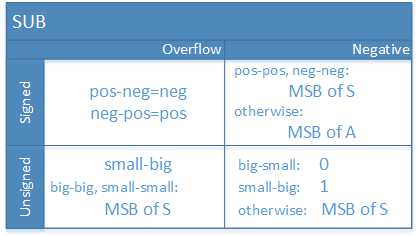
\includegraphics[width=0.5\textwidth]{images/sub_v_n.png}
                \caption{\label{fig:sub_v_n}SUB中的Overflow和Negative}
            \end{figure}
            图中的缩写含义同上。

            \paragraph*{CMP模块}
            CMP模块直接根据ARITH模块产生的Zero, Overflow, Negative进行关系判断。

            \paragraph*{LOGIC模块}
            LOGIC模块直接根据ALUFun[3:0]指定的逻辑运算进行运算。

            \paragraph*{SHIFT模块}
            将移位操作拆分为16位移位、8位移位、4位移位、2位移位、1位移位,分别用Shamt的每一个bit位控制,组合产生最后的运算结果。

        \subsection{寄存器堆、指令存储器、数据存储器和外设 \protect\footnote{作者:王晗}}
            \paragraph*{寄存器堆}
                直接采用reg [31:0] RF\_DATA[31:1]实现,注意RF\_DATA[0]不存在,读取时直接返回0。
            \paragraph*{指令存储器}
                将机器码以十六进制文本的形式存放在.rom文件中,使用\$readmemh系统任务初始化一个大小为256words的只读存储器。
            \paragraph*{数据存储器}
                由于数据存储器容量设计为256words,因此寻址时只根据address[9:2]寻址。 \\
                另外,\texttt{0x40000000}开始的地址用于外设编址,因此数据存储器不对\texttt{0x40000000}开始的地址进行读写操作。
            \paragraph*{其他外设}
                定时器、LED、Switch参考老师提供的样例代码直接在Peripheral.v中实现,UART使用春季学期第四次实验的UART发送和接收模块,将发送模块中Tx\_Status的定义取反,即1表示发送端忙碌。UART的控制同样在Peripheral.v中实现,当\texttt{0x40000018}写入要发送的数据时,串口控制器自动产生一个发送使能信号。

        \subsection{控制器和ALU控制器 \protect\footnote{作者:王晗}}
            控制单元采用两级控制的实现方法,在主控制器中根据OpCode和Funct产生PCSrc、RegWrite、RegDst、MemRead、MemWrite、MemToReg、ALUSrc1、ALUSrc2、ExtOp、LuOp、ALUOp等控制信号,其中ALUOp 经过ALU控制器进一步解码生成ALUFunc、Signed信号,控制ALU的运算,其余信号控制数据通路中的多路选择器。控制器还产生了UndefinedInst信号,用于识别未定义指令的异常。

            在单周期CPU中,PCSrc信号位宽为2,分别指示从PC+4、Branch Target、Jump Target、Jump Register取出下一个指令地址,当发生中断或异常时,由Single-Cycle Core直接跳转至中断或异常服务程序入口。在流水线CPU中,为了方便流水线寄存器操作,将PCSrc信号位宽扩展至3,当发生中断或异常,PCSrc变为100或101,指示中断或异常服务程序入口。

        \subsection{单周期数据通路 \protect\footnote{作者:王晗}}
            \begin{figure}[H]
                \centering
                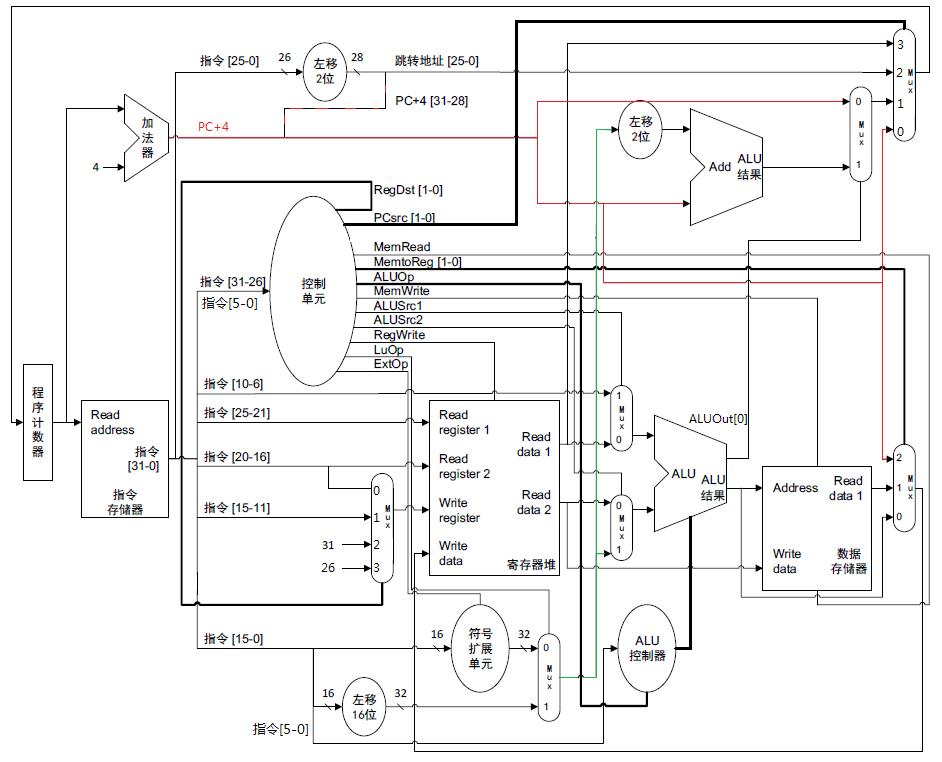
\includegraphics[width=0.95\textwidth]{images/singlecycle_datapath.png}
                \caption{\label{fig:singlecycle_datapath}单周期数据通路}
            \end{figure}

            \begin{enumerate}
                \begin{item}
                    当没有中断或异常时,根据PCSrc取出下一个PC地址,并读取指令;否则跳转至中断或异常服务程序。
                \end{item}
                \begin{item}
                    RegDst控制写入的目标寄存器:R型指令写入Rd;I型指令写入Rt;jal/jalr指令写入\$31;中断或异常写入\$26。
                \end{item}
                \begin{item}
                    ExtOp控制立即数的符号扩展或无符号扩展。
                \end{item}
                \begin{item}
                    LuOp控制立即数左移16位,用于lui指令。
                \end{item}
                \begin{item}
                    ALUSrc1用于选择RegReadData1或Shamt作为ALU的第一个操作数,ALUSrc2用于选择RegReadData2或立即数作为ALU的第二个操作数。
                \end{item}
                \begin{item}
                    MemRead、MemWrite控制外设和数据存储器的读写。
                \end{item}
                \begin{item}
                    MemToReg用于选择写入寄存器的数据来源:运算指令来源为ALU输出,lw指令来源为MemReadData,jal/jalr/中断/异常来源为PC+4。
                \end{item}
                \begin{item}
                    PC的最高位为监督位,不用于寻址。当PC[31]=1时为内核态,禁止中断请求;当PC[31]=0时为正常态,允许中断请求。Reset、异常、中断可以将PC[31]置1,jr、jalr可以将PC[31]清零。
                \end{item}
            \end{enumerate}

        \subsection{流水线数据通路 \protect\footnote{作者:王晗}}
            \begin{figure}[H]
                \centering
                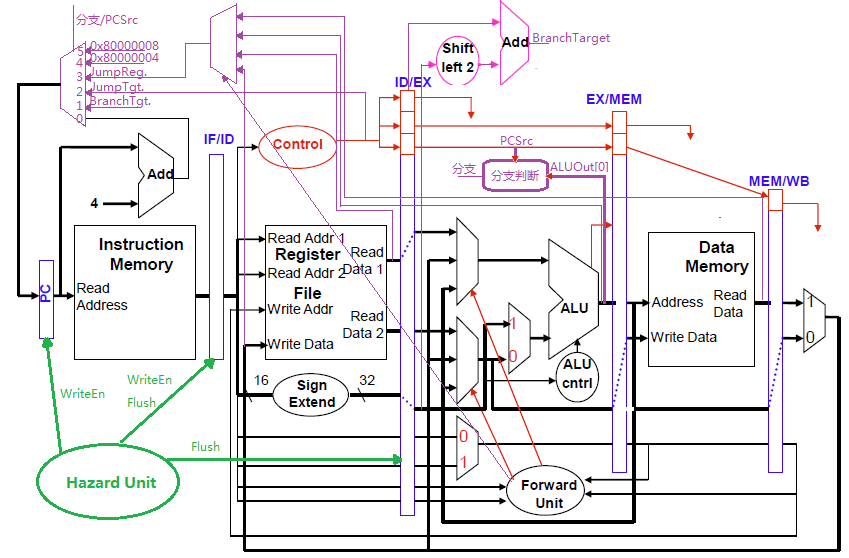
\includegraphics[width=0.95\textwidth]{images/pipeline_datapath.png}
                \caption{\label{fig:pipeline_datapath}流水线数据通路}
            \end{figure}
            \begin{enumerate}
                \begin{item}
                    在单周期数据通路的基础上添加流水线寄存器。
                \end{item}
                \begin{item}
                    添加数据转发单元,从EX/MEM或MEM/WB寄存器转发数据,解决ALU运算中的数据关联问题。
                \end{item}
                \begin{item}
                    完善数据转发单元,从ALUOut、MemReadData、RegWriteData转发数据,解决jr指令的数据关联问题。
                \end{item}
                \begin{item}
                    添加冒险检测单元,对存在load-use竞争的指令阻塞一个周期,禁止PC寄存器写入、清空ID/EX寄存器。
                \end{item}
                \begin{item}
                    完善冒险检测单元,在EX阶段进行分支时,需要清空IF/ID和ID/EX寄存器。
                \end{item}
                \begin{item}
                    完善冒险检测单元,在ID阶段进行跳转时, 需要清空IF/ID寄存器。
                \end{item}
            \end{enumerate}

        \subsection{汇编代码 \protect\footnote{作者:耿天毅}}

        \subsection{汇编器 \protect\footnote{作者:耿天毅}}

    \section{关键代码及文件清单}
        \subsection{寄存器堆的读写\protect\footnote{作者:王晗}}
            寄存器堆在同一周期对同一个寄存器先写再读不会引起数据冒险,为了实现这个目的,先对读取的寄存器地址做判断,如果读取地址为0,则返回0;如果读取地址和写入地址相同,则返回写入的值;其他情况返回寄存器堆中相应寄存器的值。
            \begin{Verbatim}[frame=lines,numbers=left,stepnumber=5,label={regfile.v}]
        assign data1 =  (addr1==5'b0)  ?  32'b0 :
                        (addr1==addr3) ?  data3 :
                        RF_DATA[addr1];
            \end{Verbatim}

        \subsection{数据转发单元\protect\footnote{作者:王晗}}
            对于ALU运算的指令,输入数据来自寄存器堆时,可能存在数据冒险。为了解决这个问题,可以从EX/MEM或MEM/WB寄存器转发数据到ALU 输入端。从EX/MEM转发的条件是前一条指令需要写非\$0寄存器,且写入地址和欲读取地址相等;从MEM/WB转发的条件是前两条指令需要写非\$0寄存器,欲读取的地址和写入地址相等,并且不能从前EX/MEM就近转发。
            \begin{Verbatim}[frame=lines,numbers=left,stepnumber=5,label={ForwardUnit.v}]
        if (EX_MEM_RegWrite == 1'b1 &&
        	EX_MEM_RegWriteAddr != 5'h00 &&
        	EX_MEM_RegWriteAddr == ID_EX_InstRs)
        		ForwardA = 2'b10;
        else if (MEM_WB_RegWrite == 1'b1 &&
        		MEM_WB_RegWriteAddr != 5'h00 &&
        		MEM_WB_RegWriteAddr == ID_EX_InstRs)
        			ForwardA = 2'b01;
        	else
        			ForwardA = 2'b00;
        //ForwardB is similar to this.
            \end{Verbatim}

            对于jr指令,同样存在数据冒险。由于跳转操作在ID阶段完成,如果检测到jr的目标寄存器和ID\_EX段写入寄存器相同,需要从ALUOut 转发数据;如果目标寄存器和EX\_MEM段写入寄存器相同,需要从MemReadData转发数据;如果目标寄存器和MEM\_WB段写入寄存器相同,则需要从RegWriteData转发数据。
            \begin{Verbatim}[frame=lines,numbers=left,stepnumber=5,label={ForwardUnit.v}]
        if (ID_PCSrc == 3'b011 && IF_ID_InstRs == ID_EX_RegWriteAddr
            && ID_EX_RegWriteAddr != 0 && ID_EX_RegWrite)
            ForwardJr = 2'b01;
        else if (ID_PCSrc == 3'b011 &&
                IF_ID_InstRs != ID_EX_RegWriteAddr &&
                IF_ID_InstRs == EX_MEM_RegWriteAddr &&
                EX_MEM_RegWrite &&
                EX_MEM_RegWriteAddr != 0)
                    ForwardJr = 2'b10;
                else if (ID_PCSrc == 3'b011 &&
                        IF_ID_InstRs != ID_EX_RegWriteAddr &&
                        IF_ID_InstRs != EX_MEM_RegWriteAddr &&
                        IF_ID_InstRs == MEM_WB_RegWriteAddr &&
                        MEM_WB_RegWriteAddr != 0 &&
                        MEM_WB_RegWrite)
                            ForwardJr = 2'b11;
                    else
                        ForwardJr = 2'b00;
            \end{Verbatim}

        \subsection{冒险检测单元\protect\footnote{作者:王晗}}
            对于load指令,需要阻塞一个周期,即在禁止PC寄存器、IF\_ID流水线寄存器写入,并清空ID\_EX流水线寄存器;\\
            对于跳转指令,在ID段完成正确的跳转,因此IF段的指令是错误的,需要清空IF\_ID流水线寄存器;\\
            对于分支指令,在EX段完成分支判断,因此如果成功跳转,IF、ID段的指令均是错误的,需要清空IF\_ID和ID\_EX流水线寄存器。
            \begin{Verbatim}[frame=lines,numbers=left,stepnumber=5,label={HazardUnit.v}]
    //参见/pipeline/HazardUnit.v
            \end{Verbatim}

            在清空寄存器时,为了保证jal/jalr/中断/异常写入寄存器堆的PC+4保持正确,我们采用了如下策略:
            \begin{enumerate}
              \item 如果ID\_EX寄存器清空,表明一条指令被抛弃,需要将ID\_EX\_PC\_plus\_4的值减4;
              \item 如果IF\_ID寄存器清空且ID\_EX不清空,表明一条指令被抛弃,需要将IF\_ID\_PC\_plus\_4的值减4;
              \item 如果IF\_ID和ID\_EX寄存器同时清空,表明两条指令被抛弃,需要将IF\_ID\_PC\_plus\_4的值减8。
            \end{enumerate}

        \subsection{UART输入\protect\footnote{作者:耿天毅}}

        \subsection{最大公约数\protect\footnote{作者:耿天毅}}

        \subsection{数码管译码\protect\footnote{作者:耿天毅}}

        \subsection{UART输出\protect\footnote{作者:耿天毅}}

        \subsection{文件清单}
            \begin{longtable}{l|ll}
                \toprule
                Directory & File & Description \\
                \midrule
                \endhead
                \bottomrule
                \endfoot
                /assembler & /MIPSAssembler.py & Python编写的汇编器 \\
                & /MIPScode\_singlecycle.asm & UART收发、求最大公约数、数码管译码 \\
                & /MIPScode\_singlecycle.rom & 汇编结果 \\
                & /MIPScode\_pipeline.asm & 在单周期基础上延长定时器周期 \\
                & /MIPScode\_pipeline.rom & 汇编结果 \\
                \midrule
                /ALU & /ALU.v & ALU顶层模块 \\
                & /ADD.v & 加法器 \\
                & /SUB.v & 减法器 \\
                & /ARITH.v & 算术运算单元 \\
                & /CMP.v & 比较运算单元 \\
                & /LOGIC.v & 逻辑运算单元 \\
                & /SHIFT.v & 移位运算单元 \\
                \midrule
                /single\_cycle & /ALU/* & ALU, 同上 \\
                & /Controller/Controller.v & 控制单元 \\
                & /Controller/ALUController.v & ALU控制单元 \\
                & /InstructionROM/rom.v & 指令存储器 \\
                & /Peripheral/Peripheral.v & 外设顶层模块 \\
                & /Peripheral/DataMem.v & 数据存储器 \\
                & /Peripheral/digitube\_scan.v & 扫描方式工作的数码管 \\
                & /Peripheral/uart* & UART相关模块 \\
                & /RegFile/regfile.v & 寄存器堆 \\
                & /clk\_gen.v & 分频模块 \\
                & /single\_cycle\_core.v & 单周期CPU内核 \\
                & /single\_cycle.v & 单周期CPU顶层模块 \\
                & /single\_cycle\_tb.v & 单周期CPU TestBench \\
                \midrule
                /pipeline & /ALU/* & ALU, 同上 \\
                & /Controller/Controller.v & 控制单元 \\
                & /Controller/ALUController.v & ALU控制单元 \\
                & /InstructionROM/rom.v & 指令存储器 \\
                & /Peripheral/* & 外设,同上 \\
                & /RegFile/regfile.v & 寄存器堆 \\
                & /RegFile/PC\_reg.v & PC寄存器 \\
                & /RegFile/IF\_ID\_reg.v & IF\_ID流水线寄存器 \\
                & /RegFile/ID\_EX\_reg.v & ID\_EX流水线寄存器 \\
                & /RegFile/EX\_MEM\_reg.v & EX\_MEM流水线寄存器 \\
                & /RegFile/MEM\_WB\_reg.v & MEM\_WB流水线寄存器 \\
                & /ForwardUnit.v & 数据转发单元 \\
                & /HazardUnit.v & 冒险检测单元 \\
                & /pipeline\_core.v & 流水线CPU内核 \\
                & /pipeline.v & 流水线CPU顶层模块 \\
                & /pipeline\_tb.v & 流水线CPU TestBench \\
            \end{longtable}

    \section{仿真结果及分析}
        \subsection{单周期LED、Switch外设}
            如Figure~\ref{fig:singlecycle_ledswitch}所示,从switch读入\texttt{0x4a},再将\texttt{0x4a}输出至led。
            \begin{figure}[H]
                \centering
                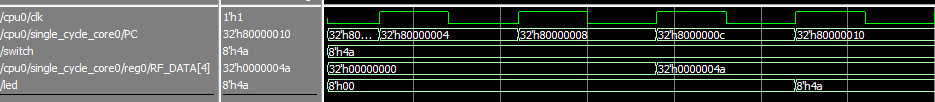
\includegraphics[width=\textwidth]{images/singlecycle_ledswitch.png}
                \caption{\label{fig:singlecycle_ledswitch}单周期LED、Switch外设}
            \end{figure}

        \subsection{\label{testdigi}单周期定时器、七段数码管}
            首先利用jr指令清空PC[31],从而允许中断(如Figure~\ref{fig:singlecycle_digi1}所示)。
            \begin{figure}[H]
                \centering
                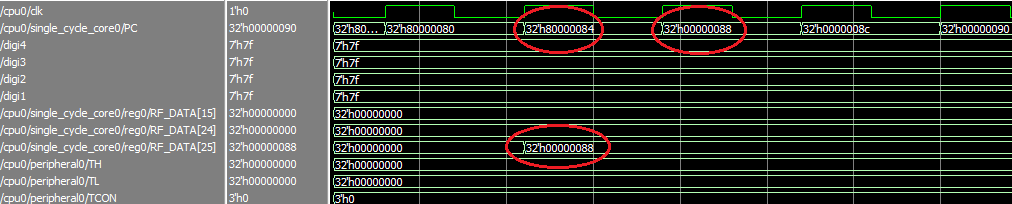
\includegraphics[width=\textwidth]{images/singlecycle_digi1.png}
                \caption{\label{fig:singlecycle_digi1}清空PC[31]}
            \end{figure}
            然后对定时器置数,启动定时器(如Figure~\ref{fig:singlecycle_digi2}所示)。
            \begin{figure}[H]
                \centering
                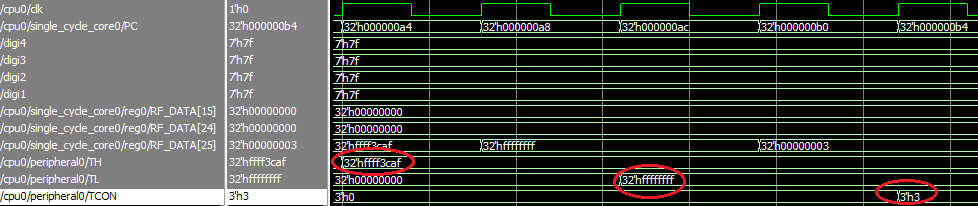
\includegraphics[width=\textwidth]{images/singlecycle_digi2.png}
                \caption{\label{fig:singlecycle_digi2}启动定时器}
            \end{figure}
            发生定时器中断时,先禁用定时器中断,改变一个数码管的值,再启用定时器中断(如Figure~\ref{fig:singlecycle_digi3}所示)。
            \begin{figure}[H]
                \centering
                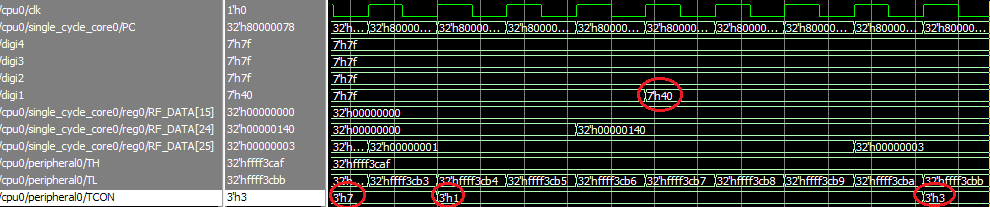
\includegraphics[width=\textwidth]{images/singlecycle_digi3.png}
                \caption{\label{fig:singlecycle_digi3}定时器中断}
            \end{figure}

        \subsection{单周期串口}
            如Figure~\ref{fig:singlecycle_uart}所示,从串口接收数据,加1,再通过串口返回。
            \begin{figure}[H]
                \centering
                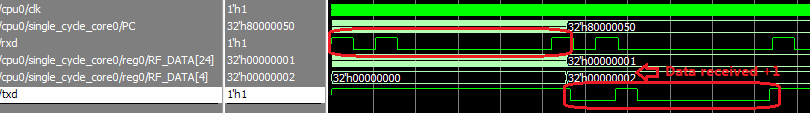
\includegraphics[width=\textwidth]{images/singlecycle_uart.png}
                \caption{\label{fig:singlecycle_uart}单周期串口}
            \end{figure}

        \subsection{单周期完整程序}
            我们先在MARS模拟器上进行了仿真(如Figure~\ref{fig:singlecycle_full1}所示),\$s1=125、\$s2=25为两个输入参数,\$s3=25为输出结果,最大公约数计算正确。
            \begin{figure}[H]
                \centering
                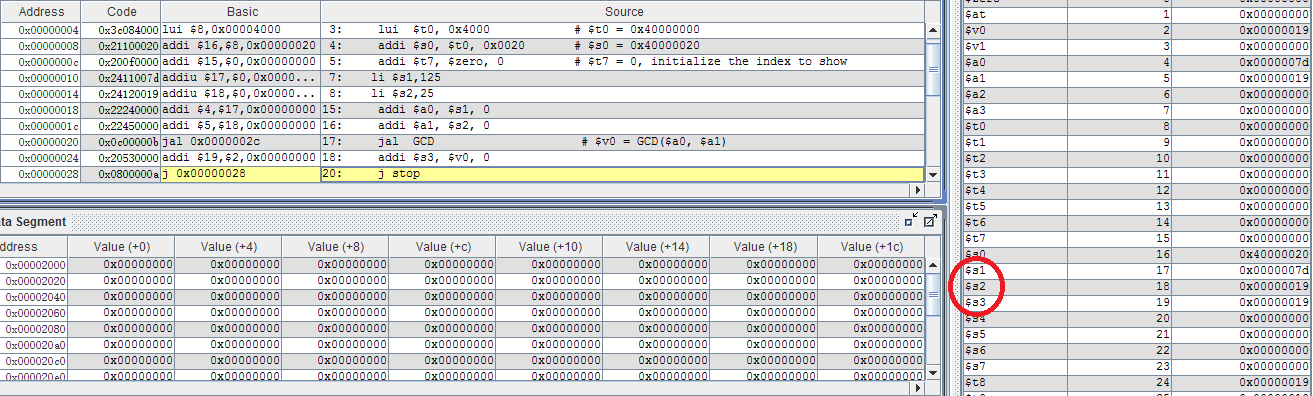
\includegraphics[width=\textwidth]{images/singlecycle_full1.png}
                \caption{\label{fig:singlecycle_full1}MARS仿真器仿真结果}
            \end{figure}
            如Figure~\ref{fig:singlecycle_full2}所示,从UART读入两个操作数,分别存放至\$s1、\$s2,最大公约数运算结果存放到\$s3,通过LED显示,同时经UART输出。
            \begin{figure}[H]
                \centering
                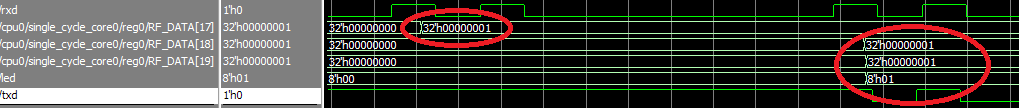
\includegraphics[width=\textwidth]{images/singlecycle_full2.png}
                \caption{\label{fig:singlecycle_full2}单周期完整程序运行结果}
            \end{figure}

        \subsection{流水线数据通路}
            如Figure~\ref{fig:pipeline_datapathtest}所示,将\$1置1,5个时钟周期后1被写入寄存器堆;
            两个空指令(nop)后,将\$1加1并存入\$2,这时\$1的写入和读取发生在同一个时钟周期内。
            \begin{figure}[H]
                \centering
                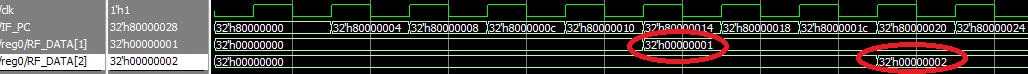
\includegraphics[width=\textwidth]{images/pipeline_datapathtest.png}
                \caption{\label{fig:pipeline_datapathtest}流水线数据通路测试}
            \end{figure}

        \subsection{流水线数据转发}
            连续执行如下三条指令:
            \begin{Verbatim}[frame=lines,numbers=left,stepnumber=5,label={test\_dataforward.asm}]
            addi $1,$0,1
            add $2,$1,2
            add $3,$1,3
            \end{Verbatim}
            这三条指令之间存在数据关联,需要Data-Forward Unit正常工作才能正确执行。

            仿真结果如Figure~\ref{fig:pipeline_dataforwardtest}所示:
            \begin{figure}[H]
                \centering
                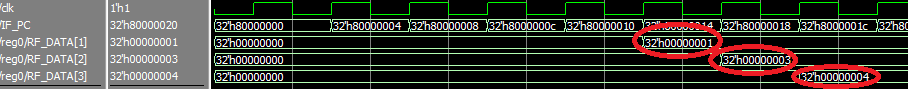
\includegraphics[width=\textwidth]{images/pipeline_dataforwardtest.png}
                \caption{\label{fig:pipeline_dataforwardtest}流水线数据转发测试}
            \end{figure}

        \subsection{流水线竞争冒险}
            执行下列指令:
            \begin{Verbatim}[frame=lines,numbers=left,stepnumber=5,label={test\_loaduse.asm}]
            addu $1, $0, $0
            lui $1, 0x4000
            lw $2, 16($1)
            addi $2, $2, 1
            sw $2, 12($1)
            \end{Verbatim}
            lui和lw指令之间存在数据关联,lw和addi指令之间存在load-use竞争,需要阻塞一个周期。
            \begin{figure}[H]
                \centering
                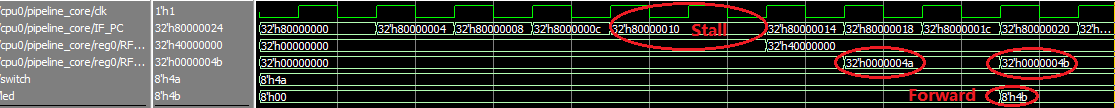
\includegraphics[width=\textwidth]{images/pipeline_loadusetest.png}
                \caption{\label{fig:pipeline_loadusetest}load-use冒险测试}
            \end{figure}
            如Figure~\ref{fig:pipeline_loadusetest}所示,流水线被成功阻塞,运算结果正确。

        \subsection{流水线定时器、七段数码管}
            在流水线CPU上运行Section~\ref{testdigi}中的汇编代码,测试流水线中的分支、跳转和中断。

            如Figure~\ref{fig:pipeline_digitest1}所示,Jump和Jump-to-Register均工作正常,其中jr指令采用dataforward提前完成了跳转。
            \begin{figure}[H]
                \centering
                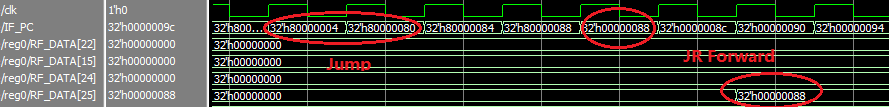
\includegraphics[width=\textwidth]{images/pipeline_digitest1.png}
                \caption{\label{fig:pipeline_digitest1}流水线中的跳转}
            \end{figure}
            如Figure~\ref{fig:pipeline_digitest2}所示,中断发生时,程序跳转至中断服务程序入口\texttt{0x80000004}。
            \begin{figure}[H]
                \centering
                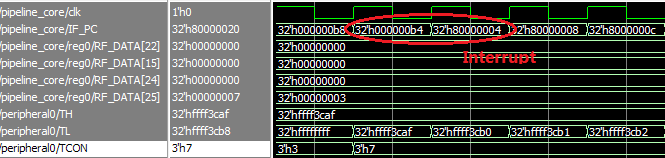
\includegraphics[width=0.8\textwidth]{images/pipeline_digitest2.png}
                \caption{\label{fig:pipeline_digitest2}流水线中的中断}
            \end{figure}
            如Figure~\ref{fig:pipeline_digitest3}所示,\$24记录的是下一个需要点亮的数码管,程序根据\$24的值进行分支,点亮不同的数码管,实现译码输出。
            \begin{figure}[H]
                \centering
                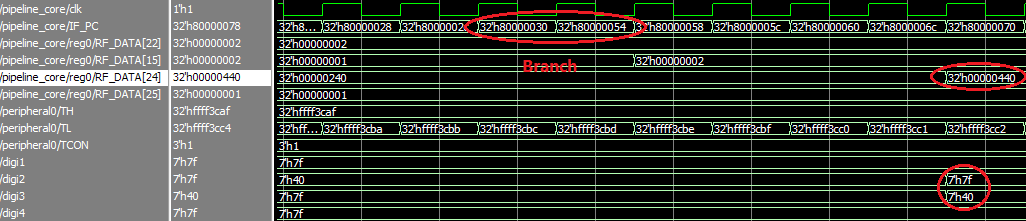
\includegraphics[width=\textwidth]{images/pipeline_digitest3.png}
                \caption{\label{fig:pipeline_digitest3}流水线中的分支}
            \end{figure}

        \subsection{流水线完整程序}
            由于流水线CPU的时钟频率明显高于单周期,因此我们在流水线中去除了分频模块,并且增大了定时器计数范围。

            如Figure~\ref{fig:pipeline_full}所示,从UART读入两个操作数,分别存放至\$s1、\$s2,最大公约数运算结果存放到\$s3。
            \begin{figure}[H]
                \centering
                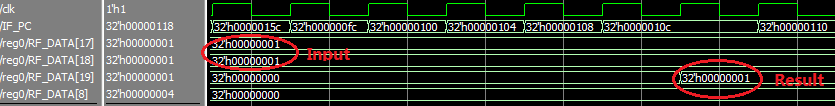
\includegraphics[width=\textwidth]{images/pipeline_full.png}
                \caption{\label{fig:pipeline_full}流水线完整程序运行结果}
            \end{figure}

    \section{综合情况}
        \begin{table}[H]
            \centering
            \begin{tabular}{c|lr}
              \toprule
              Version & Specification & Value \\
              \midrule
              Single Cycle  & Total combinational functions & 8,990 / 33,216 (27\%) \\
                            & Dedicated logic registers & 9,435 / 33,216 (28\%) \\
                            & Max frequency & 31.81 MHz \\
                            & Setup time & 8.564 ns \\
                            & Hold time & 0.391 ns \\
              \midrule
              Pipeline  & Total combinational functions & 9,699 / 33,216 (29\%) \\
                        & Dedicated logic registers & 9,982 / 33,216 (30\%) \\
                        & Max frequency & 63.36 MHz \\
                        & Setup time & 4.218 ns \\
                        & Hold time & 0.391 ns \\
              \bottomrule
            \end{tabular}
        \end{table}


    \section{硬件调试情况}
        \begin{enumerate}
          \item 在测试定时器和七段数码管时,汇编代码的最后一句是stop: j stop,然而中断服务程序返回后程序并未停留在此处。分析数据通路后发现,\$26寄存器存储的是PC+4地址,但是中断发生时PC语句并没有正确执行,因此中断服务程序返回前需要将\$26的值减4,否则程序将会跳过PC语句。
          \item 理论课讨论的MIPS子集中并未包含jr指令,做流水线设计时也没有考虑到jr引起的数据冒险。硬件调试中我们发现,(a)中提出先将\$26的值减4再跳转,这样的设计在流水线中无法正确实现,因此我们决定增加jr指令的数据转发单元。
          \item 执行完整的最大公约数程序时,我们发现如果不开启定时器,则UART工作正常;一旦开启定时器,UART就会在Rx Status无效时继续读数。仔细排查发现,问题的原因是定时器中断服务程序中使用的\$t0寄存器和主程序中的\$t0寄存器存在冲突。更换临时寄存器后,问题得到了解决。
        \end{enumerate}

    \section{心得体会}
        很早就听说过大二暑假的MIPS处理器设计,尽管任务艰巨,但我们仍然十分期待。

        3天单周期、3天流水线,我们用最快的速度和严谨的代码风格高质量地完成了处理器设计实验,并且在验收时得到了老师和助教的好评。这6 天的时间里,我们有过返工,例如陈志杰同学最初编写的ALU,代码风格欠佳,缺乏注释,大量使用x、y、z、t作为变量,给后续的联调造成了许多困难;这6天时间里,我们也有过讨论,Coding.Net讨论区、微信群、寝室都是我们讨论的场所,小组内外的讨论常常持续到凌晨……

        实验结束了,看得见的是Coding.Net上一行行commit记录,看不见的是实验中对CPU的深入理解和收获。

\end{document}
